
%aca va el ejercicio

Se tomaron los datos de m\'aximos y m\'inimos de las entradas y salidas para los distintos estados de las hojas de datos de los circuitos en cuesti\'on, y se exhiben en el cuadro \ref{tab:datos74}.
\begin{table}[H]
\begin{tabular}{|l|l|l|l|l|l|l|}
\hline
                                                                            & Vcc                                                        & Voltage (25 C)                                              & Vcc         & Voltage (25 C) & Vcc      & Voltage (25 C)   \\ \hline
                                                                      & \multicolumn{2}{l|}{74HC02}                                                                                              & \multicolumn{2}{l|}{74HCT02} & \multicolumn{2}{l|}{74LS02} \\ \hline
\begin{tabular}[c]{@{}l@{}}Minimum HIGH Level\\ Input Voltage\end{tabular}  & \begin{tabular}[c]{@{}l@{}}2.0V\\ 4.5V\\ 6.0V\end{tabular} & \begin{tabular}[c]{@{}l@{}}1.5V\\ 3.15V\\ 4.2V\end{tabular} & 4.5V a 5.5V & 2V             & 4.75V    & 2V               \\ \hline
\begin{tabular}[c]{@{}l@{}}Maximum LOW Level\\ Input Voltage\end{tabular}   & \begin{tabular}[c]{@{}l@{}}2.0V\\ 4.5V\\ 6.0V\end{tabular} & \begin{tabular}[c]{@{}l@{}}0.5V\\ 1.35V\\ 1.8V\end{tabular} & 4.5V a 5.5V & 0.8V           & 4.75V    & 0.8V             \\ \hline
\begin{tabular}[c]{@{}l@{}}Minimum HIGH Level\\ Output Voltage\end{tabular} & \begin{tabular}[c]{@{}l@{}}2.0V\\ 4.5V\\ 6.0V\end{tabular} & \begin{tabular}[c]{@{}l@{}}1.9V\\ 4.4V\\ 5.9V\end{tabular}  & 4.5V a 5.5V & 4.4V           & 4.75V    & 2.7V             \\ \hline
\begin{tabular}[c]{@{}l@{}}Maximum LOW Level\\ Output Voltage\end{tabular}  & \begin{tabular}[c]{@{}l@{}}2.0V\\ 4.5V\\ 6.0V\end{tabular} & \begin{tabular}[c]{@{}l@{}}0.1V\\ 0.1V\\ 0.1V\end{tabular}  & 4.5V a 5.5V & 0.1V           & 4.75V    & 0.5V             \\ \hline
\end{tabular}
\caption{Tabla de informaci\'on obtenida de las hojas de datos}
\label{tab:datos74}
\end{table}

Como se ilustra en las figuras para los cuatro casos planteados, s\'olo habr\'ia problemas si se intenta conectar un transistor HC a la salida de un LS: la salida alta del LS puede caer en la regi\'on indeterminada de la entrada del HC, y sin que falle ning\'un componente fallar\'ia el circuito.

En todos los dem\'as casos se genera un margen de error para las entradas de los transistores.


\begin{figure}[h]% este es para caption arriba o abajo
  \centering
    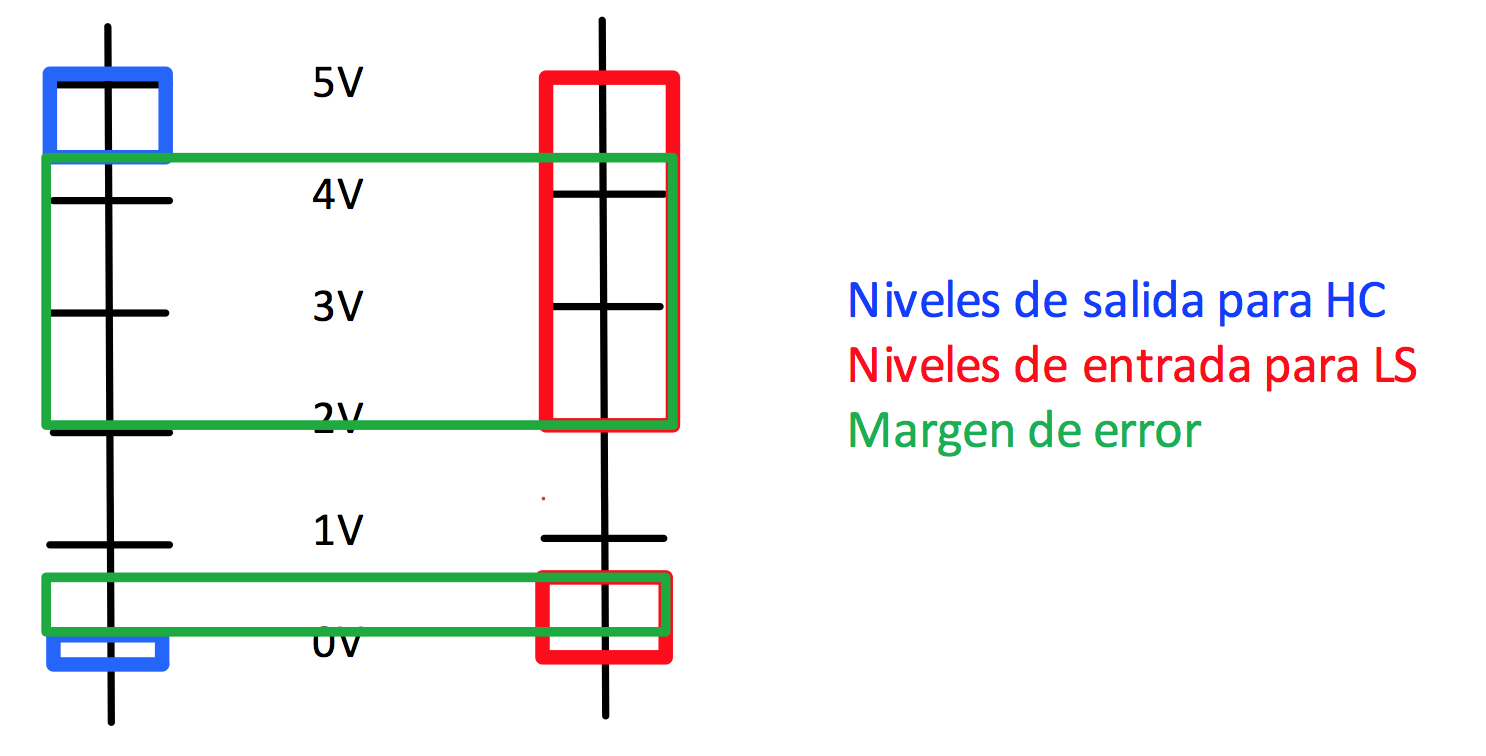
\includegraphics[width=0.5\textwidth]{HC->LS}
    \caption{Niveles de tensi\'on para caso HC->LS.} %caption abajo
\end{figure}

\begin{figure}[h]% este es para caption arriba o abajo
  \centering
    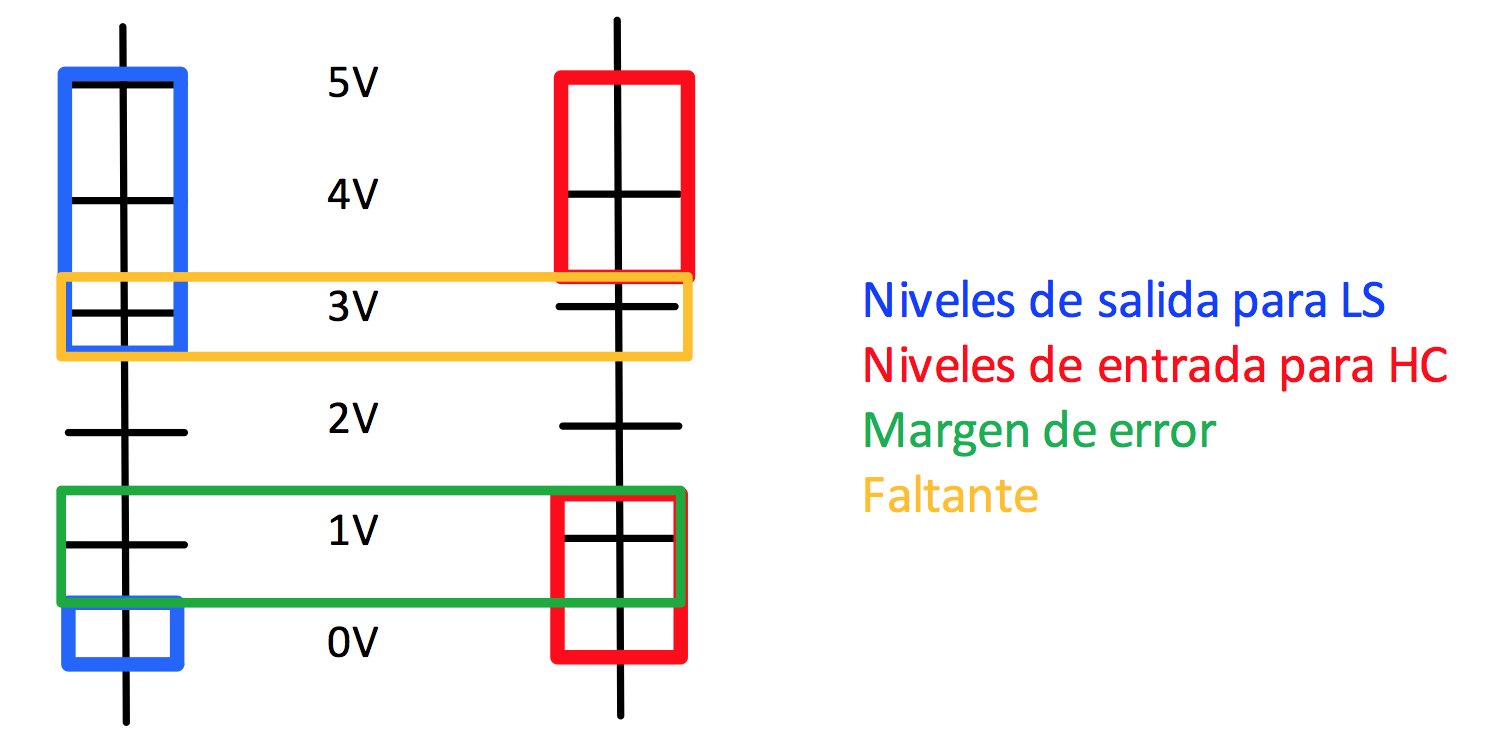
\includegraphics[width=0.5\textwidth]{LS->HC}
    \caption{Niveles de tensi\'on para caso LS->HC.} %caption abajo
\end{figure}

\begin{figure}[h]% este es para caption arriba o abajo
   \centering
    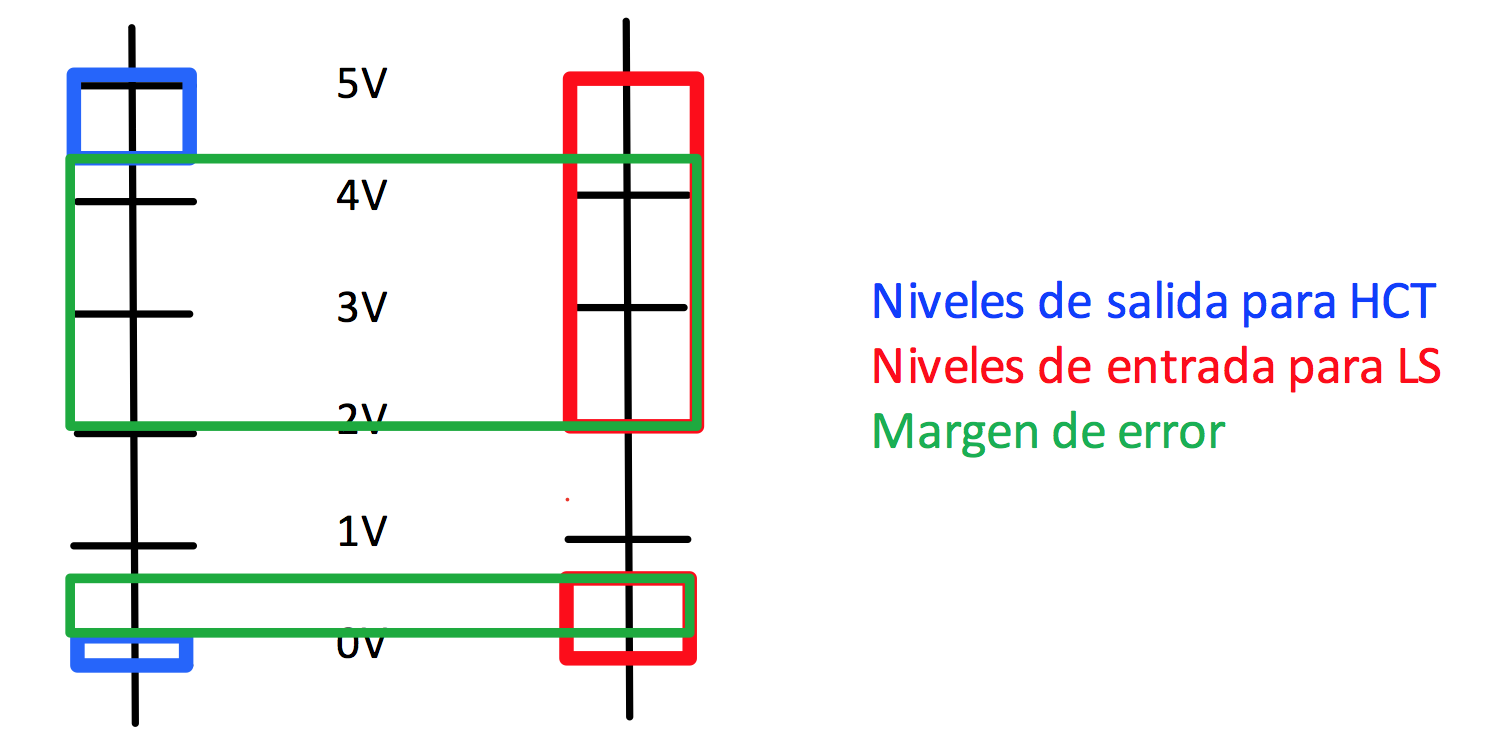
\includegraphics[width=0.5\textwidth]{HCT->LS}
    \caption{Niveles de tensi\'on para caso HCT->LS.} %caption abajo
\end{figure}

\begin{figure}[h]% este es para caption arriba o abajo
   \centering
    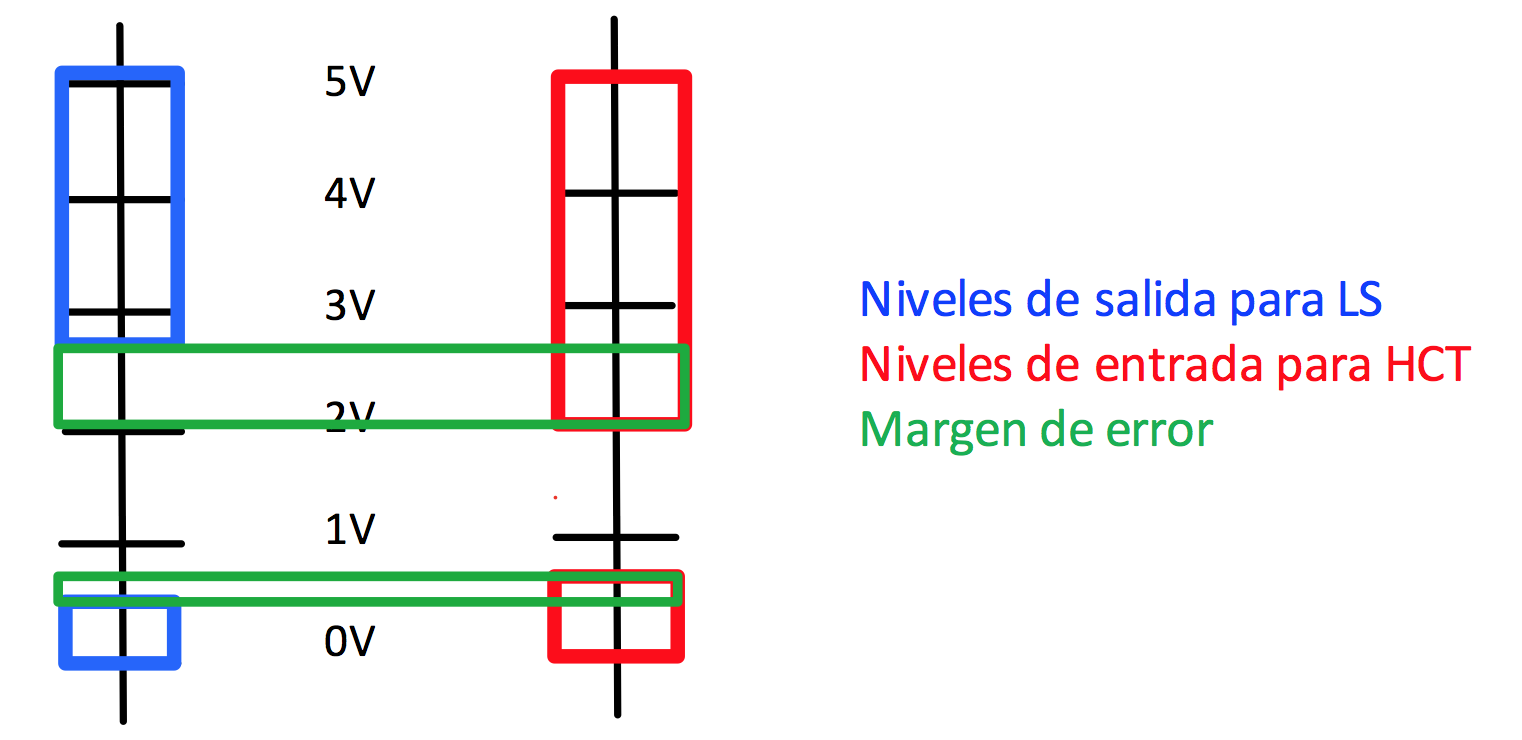
\includegraphics[width=0.5\textwidth]{LS->HCT}
    \caption{Niveles de tensi\'on para caso LS->HCT.} %caption abajo
\end{figure}

Procedimos a alimentar una compuerta del integrado LS02 con la salida de una misma compuerta pero del integrado HC02, y luego alimentamos de la misma manera pero en sentido inverso. Pudimos notar que hay zonas donde el circuito armado no deber\'ia andar de forma \'optima por el margen de ruido que manejan las distintas compuertas pero funciona igual ya que la ca\'ida de tensi\'on en el LS02 no es tan grande y alcanza a caer cerca del l\'imite del HC02 con 4,2V aproximadamente que es el m\'inimo del estado HIGH para el HC02. Si hubiera sido menor el valor de la tensi\'on no hubi\'eramos obtenido alguna salida por lo marcado en las hojas de datos.
\newline
El \textbf{fan-out} est\'a determinado por la cantidad de corriente que puede aceptar en la entrada cada CI y es la cantidad de pines que puede alimentar un CI con alguna de sus salidas. En la tecnolog\'ia CMOS(HC) seg\'un su hoja de dato acepta 20mA como m\'aximo, mientras que la tecnolog\'ia TTL(LS) acepta 0,4mA como m\'aximo en la entrada y 8mA en la salida. Haciendo las cuentas directas de estos casos, con la salida de un integrado LS puedo alimentar hasta 20 entradas LS, mientras que con un HC puedo alimentar 50 entradas LS. Cabe destacar que en la hoja de datos que brinda el fabricante solo asegura el funcionamiento de hasta 10 pines LS-TTL con una salida del HC, el cual debe ser para el peor caso que puede surgir para este integrado.
\newline
Al hacer las mediciones alimentando con el HCT y notamos un comportamiento mejor en cuanto la alimentaci\'on del LS02, ya que la tecnolog\'ia HCT es a base de CMOS pero tiene una gran tolerancia con la tecnolog\'ia TTL en cuanto a los valores de tensi\'on.



\iffalse
Seccion de cosas utiles para agregar

texto----------------------------
\textit[texto en negrita]




listas --------------------------------------------------
\begin{list_type}  
\item The first item 
\item The second item 
\item The third etc \ldots 
\end{list_type}

list_type es:
itemize for a bullet list
enumerate for an enumerated list and
description for a descriptive list.

ejemplo listas anidadas-----------------------------------------------

\begin{enumerate}
\item The first item
\begin{enumerate}
\item Nested item 1
\item Nested item 2
\end{enumerate}
\item The second item
\item The third etc \ldots
\end{enumerate}

tildes-------------------------------
babel ya esta incluido, si hay que poner tildes se ponen \acute{i}
ejemplo: l\acute{i}mite

tip: escriban normal y despues hagan replace

subsecciones-------------------------------

si necesitan subsecciones le clavan un buen \subsection*{nombre}

y si estan en piolas y necesitan sub sub secciones le clavan un \subsubsection*{nombre}

quien hubiera dicho

figuras----------------------------------------

\begin{figure}[h]% este es para caption arriba o abajo
  \caption{A picture of a gull.} %caption arriba
  \centering
    \includegraphics[width=0.5\textwidth]{gull}
    \caption{A picture of a gull.} %caption abajo
\end{figure}

\begin{SCfigure} %este es para caption al costado
  \centering
  \caption{ ... caption text ... } 
  \includegraphics[width=0.3\textwidth]%
    {Giraffe_picture}% picture filename
\end{SCfigure}

para hacer que la figure se quede quietecita:

\begin{figure}[letrita_placement]

donde letrita_placement es:
h	Place the float here, i.e., approximately at the same point it occurs in the source text (however, not exactly at the spot)
t	Position at the top of the page.
b	Position at the bottom of the page.
p	Put on a special page for floats only.
!	Override internal parameters LaTeX uses for determining "good" float positions.
H	Places the float at precisely the location in the LaTeX code. Requires the float package,[1] i.e., \usepackage{float}. This is somewhat equivalent to !ht.

\fi